\documentclass[a4paper]{article}
\usepackage[a4paper, top=17mm, bottom=17mm, left=17mm, right=17mm]{geometry}
\usepackage[utf8]{inputenc}
\usepackage[T2A,T1]{fontenc}
\usepackage[colorlinks,filecolor=blue,citecolor=green,unicode,pdftex]{hyperref}
\usepackage{cmap}
\usepackage[english,russian]{babel}
\usepackage{amsmath}
\usepackage{amssymb,amsfonts,textcomp}
\usepackage{color}
\usepackage{array}
\usepackage{hhline}
\hypersetup{colorlinks=true, linkcolor=blue, citecolor=blue, filecolor=blue, urlcolor=blue, pdftitle=1, pdfauthor=, pdfsubject=, pdfkeywords=}
\usepackage[pdftex]{graphicx}
\usepackage{graphicx}
% Раскомментировать тем, у кого этот пакет есть. Шрифт станет заметно красивее.
%\usepackage{literat}
\usepackage{indentfirst}
\usepackage{multirow}
\usepackage{subfig}

\sloppy
\pagestyle{plain}

\title{Технология визуального предметно-ориентированного проектирования и разработки ПО QReal}

\author{Т.А.Брыксин \and Ю.В.Литвинов}
\date{}
\begin{document}

\maketitle
\thispagestyle{empty}

\begin{quote}
\small\noindent
В статье описывается инструментальная среда QReal, являющаяся как CASE-средством, так и позволяющая быстро создавать визуальные предметно-ориентированные языки, редакторы и генераторы исходных кодов для них. Дается описание общей архитектуры системы, основных функциональных особенностей. 
\end{quote}

\section*{Введение}

Модельно-ориентированная разработка ПО~\footnote{Model-driven development, MDD} основывается на представлении программы в виде набора моделей, описывающих ее с различных точек зрения. При этом обычно используются визуальные языки моделирования, с их помощью создаются разного уровня абстракции описания предметной области, разрабатываемой системы и взаимодействующего с ней окружения. Считается, что в целом данный подход упрощает процесс разработки и понимания системы, делает его более наглядным, снижает вероятность появления ошибок, повышает продуктивность разработчиков. Наиболее активное распространение CASE-технологий\footnote{Computer-aided software engineering}  началось в середине 90-х годов прошлого века, когда появился унифицированный язык моделирования UML\footnote{http://www.uml.org/}. К концу 90-х годов был разработан набор методологий разработки ПО (и поддерживающих их инструментариев), в том или ином виде предполагающих активное использование визуального проектирования. При этом вполне закономерно желание иметь полную автоматическую генерацию исполняемого кода по диаграммам, однако, это неизбежно приводит к жесткой формализации соответствующих графических языков. При этом использование языков общего назначения (например, Executable UML) чаще всего приводит к тому, что диаграммы теряют наглядность и простоту, становятся громоздкими и сложными для восприятия. Парадигма предметно-ориентированного моделирования (Domain-specific modeling) основывается на том факте, что чаще создание нового специального языка и решение с его помощью поставленной практической задачи можно осуществить быстрее, чем решать ту же задачу с помощью языков общего назначения (подробнее про преимущества и ограничения, появляющиеся при использовании DSM-подхода, см. в ~\cite{theBook}). Имея соответствующую инструментальную поддержку, данный подход позволяет значительно повысить уровень абстракции, но котором работают проектировщики, и увеличить производительность их труда в несколько раз ~\cite{dsm01}.

\section*{QReal}

Разработкой технологии QReal занимается научно-исследовательская группа изучения технологий визуального моделирования кафедры системного программирования Санкт-Петербургского Государственного Университета под руководством проф. А.Н. Терехова.  QReal~\cite{qreal}  изначально задумывалась как развитие технологии REAL~\cite{real}, основывающееся на использовании более современной версии языка UML --- 2.0. При этом на разрабатываемые средства накладывались требования многоплатформенности (возможность работы на наиболее популярных операционных системах MS Windows и Linux), поддержка многопользовательской разработки, возможность удаленного доступа к репозиторию системы и другая актуальная для современных сред визуальной разработки ПО функциональность. Однако, стало быстро очевидно, что создание большого числа редакторов диаграмм вручную является довольно утомительным занятием, к тому же получаемая система оказывается плохо масштабируемой. В результате в QReal были добавлены средства метамоделирования, которые позволяют быстро создавать новые редакторы, задавая описание метамоделей разрабатываемого языка и визуальное представление его элементов.


\subsection*{Архитектура}
Инфраструктуру QReal можно представить следующим образом (см. рис.~\ref{qRealArchitecture}):

\begin{itemize}
  \item Архитектура QReal основывается на шаблоне проектирования Model/View. Модель обеспечивает доступ к репозиторию, а в роли представлений выступают различные элементы пользовательского интерфейса (инспектор логических и графических моделей, редактор свойств и т.д.). 
\begin{figure} [ht]
  \begin{center}
    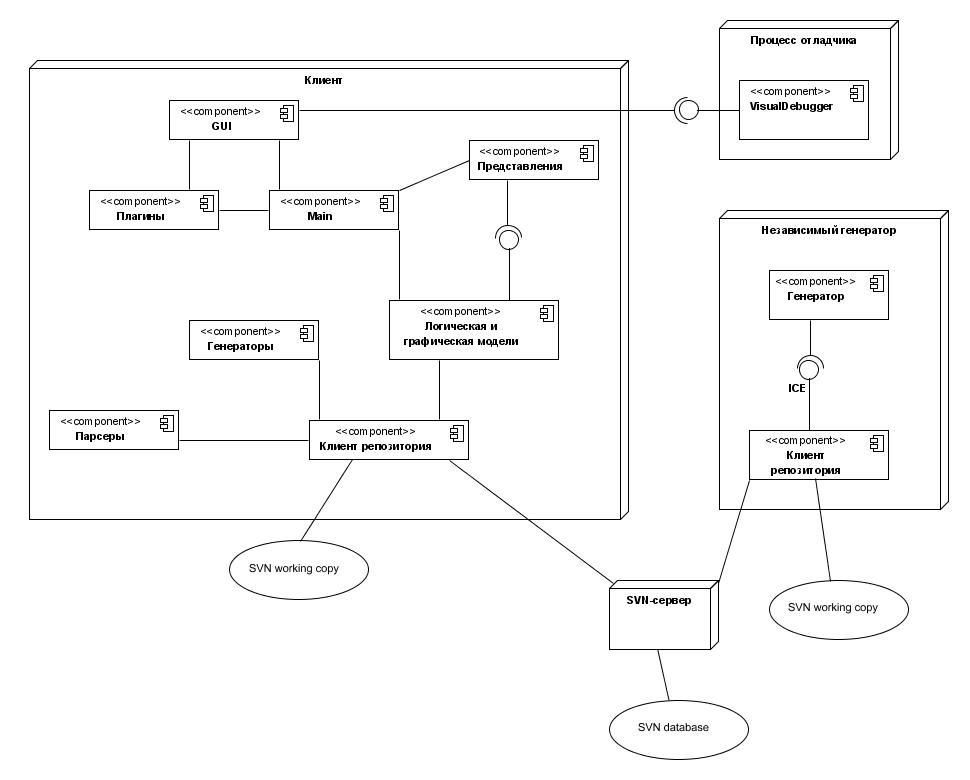
\includegraphics[width=0.7\textwidth]{01-architecture.png}
    \caption{Архитектура QReal}
    \label{qRealArchitecture}
  \end{center}
\end{figure}
  \item Ввиду того, что набор графических редакторов QReal не фиксирован, каждый визуальный редактор является подключаемым модулем. Инфраструктура CASE-системы включает в себя абстрактное ядро, реализующее общую для всех редакторов и элементов диаграмм функциональность, и подключаемых модулей, реализующих специфику конкретных редакторов. Каждый такой модуль инкапсулирует в себе информацию о наборе объектов, допустимых на диаграммах данного типа, позволяет правильно интерпретировать хранящиеся в репозитории значения атрибутов элементов и предоствляет информацию о логических правилах размещения элементов на соответствующих типах диаграмм.
  \item Для обеспечения версионирования и многопользовательской работы используется сервер Subversion. Доступ к нему осуществляется посредством клиентов репозитория, которые хранят свои модели в виде текстовых файлов, организованных в рабочую копию системы контроля версий. При старте QReal файлы моделей читаются с диска и строится объектная структура, с которой и происходит работа при манипуляциями с репозиторием. 
  \item В QReal представление и хранение данных основано на разделении графических и логических моделей. Элемент модели и его визуальное представление --- по сути разные вещи. Некоторые элементы модели могут вовсе визуального представления не иметь (например, значения перечислимых типов), некоторые наоборот, имеют только визуальное представление и на логику никак не влияют (например, просто линия или прямоугольник на диаграмме), некоторые могут иметь несколько представлений. В CASE-пакете реализованы необходимые средства, позволяющие разработчикам создавать различные представления одних и тех же логических моделей.
\end{itemize}


\subsection*{Средства метамоделирования}

В QReal реализованы два подхода, позволяющие любому заинтересованному пользователю системы, не обладающему навыками программирования и не знакомому с внутренним устройством системы, создать новый редактор диаграмм, встраиваемый в QReal.
\begin{itemize}
  \item Метамодель разрабатываемого языка описывается в виде XML-формата довольно простой структуры. Графические изображения элементов задаются с помощью текстового языка SDF, являющегося расширением языка описания векторной графики SVG~\footnote{Scalable Vector Graphics, http://www.w3.org/Graphics/SVG/}.
  \item Метамодель языка задается графически в метаредакторе QReal посредством простого визуального языка, являющего аналогом MOF~\footnote{MetaObject Facility, http://www.omg.org/mof/}. Для описания представлений элементов языка на диаграммах используется графический редактор форм, позволяющий создавать из набора примитивов векторные изображения или загружать уже готовые растровые.
\end{itemize}
Стоит отметить, что в QReal эти два подхода являются взаимозаменяемыми, поскольку XML-описание метамодели языка может быть как загружено в метаредактор, так и сгенерировано из него. 

В дополнение к метаредактору для быстрого создания трансляторов визуальных диаграмм в исходный код на некотором текстовом языке в QReal используется специальный язык описания генераторов. Так, для каждого разрабатываемого визуального языка можно задать правила обхода созданных с его помощью диаграмм и генерации кода по ним. В дальнейшем эти правила интерпретируются для конкретных диаграмм, порождая соответствующий им код на выбранном целевом языке.
  
\subsection*{Отладчик}

Для редактора блок-схем и некоторых других поведенческих диаграмм, основывающихся на сетях Петри, в QReal реализован визуальный интерпретатор, который позволяет разработчику пошагово выполнять созданные диаграммы. При этом среда на каждом шаге автоматически проверяет синтаксическую и семантическую корректность созданной диаграммы, текущий элемент или связь подсвечиваются. Стоит отметить, что разработчик может менять диаграмму прямо в процессе интерпретации, что дает дополнительные удобства для отладки созданных алгоритмов. 
  
Помимо пошаговой интерпретации, в QReal ведется работа и над полноценной отладкой сгенерированного по диаграммам исполнимого кода. Для каждого типа используемых целевых отладчиков (gdb для С/C++, pdb для Python и др.) в QReal создается отдельный модуль, предоставляющий системе запускать программу, выполнять пошаговую отладку, устанавливать точки останова, завершать процесс и выполнять другие типичные для средств отладки команды. Выполняя поданные команды, модуль отладчика сообщает о результатах обратно в QReal, передавая дополнительную информацию типа текущих значений переменных, текущего места останова и др. 
  
\subsection*{Повышение удобства использования и производительности труда}

Большое значение в QReal уделяется удобству и простоте использования инструментальных средств (usability). Так, был реализован подход, при котором создание объектов на диаграммах и связей между ними ассоциируется с определёнными жестами мышью (в общем случае каждому элементу ставится в соответствие отдельный жест), выполненный с каким-либо модификатором (в случае QReal --- с зажатой правой кнопкой мыши)~\cite{mousegestures}. При выполнении жеста в указанном месте диаграммы создается соответствующий объект. На наш взгляд данный механизм позволяет автоматизировать и ускорить наиболее часто выполняемую при проектировании диаграмм операцию --- создание элементов. Также в процессе моделирования важным является удобство работы с связями между элементами:
\begin{itemize} 
  \item В QReal связь между элементами можно создать, сделав жест мышью, начинающийся и заканчивающийся на нужных элементах. При этом если между типами этих элементов может существовать несколько ассоциаций, среда предложить выбрать нужную связь во всплывающем меню. 
  \item Точки излома ассоциаций можно добавить, просто потащив за какой-либо участок ломаной. 
  \item При выделении объекта на диаграмме вокруг него появляются несколько кружков, каждый из которых ассоциирован с видами связей, которые из данного элемента могут исходить. При нажатии на них из элемента можно “вытащить” связь. Если пользователь при этом отпускает кнопку мыши на свободном пространстве диаграммы, ему предлагается список элементов, которых можно соединить с выбранным данным типом связи. Если же кнопка мыши отпускается на существующем элементе, система проверяет, можно ли соединить эти элементы выбранным типом связи, и решает, стоит ли создавать данную ассоциацию или нет. 
\end{itemize}

\section*{Заключение}

Описанный в статье metaCASE инструментарий QReal был использован для создания ряда визуальных редакторов и генераторов исходного кода по ним: набор редакторов UML 2.1 (с генерацией в Java и C\#.NET), редактор бизнес-процессов на язке BPEL, редактор требований, ряд предметно-ориентированных решений для описания схем FPGA, интернет-сервисов для платформы Android, программ управления роботом Lego Mindstorms NXT, программ, распараллеливаемых с помощью MPI и др.

На основе полученного опыта мы полагаем, что при наличии мощной инструментальной поддержки использование предметно-ориентированных визуальных языков реализует принципиально новый подход к созданию сложных систем с довольно низким порогом вхождения для новичков и многократным увеличением производительности профессионалов. Проект QReal ставит своей целью исследование, реализацию и апробацию таких инструментов и технологий, на них основанных.

\begin{thebibliography}{9001}
  \bibitem{mousegestures} М.С. Осечкина, Т.А. Брыксин, Ю.В. Литвинов и др., Поддержка жестов мышью в мета-CASE-системах  // Системное программирование. Вып. 5. СПб.: Изд-во СПбГУ. 2010
  \bibitem{qreal} А.Н. Терехов, Т.А. Брыксин, Ю.В. Литвинов и др., Архитектура среды визуального моделирования QReal. // Системное программирование. Вып. 4. СПб.: Изд-во СПбГУ. 2009, С. 171-196
  \bibitem{real} А.Н. Терехов, К.Ю. Романовский, Д.В. Кознов и др. REAL: методология и CASE-средство для разработки систем реального времени и информационных cистем // Программирование. 1999. № 5. C. 44-52.
  \bibitem{theBook} Kelly, S., Tolvanen, J.-P. Domain-Specific Modeling: Enabling Full Code Generation // Wiley-IEEE Computer Society Press. 2008. 448 pp.
  \bibitem{dsm01} Kelly, S., Tolvanen, J.-P. Visual domain-specific modeling: benefits and experiences of using metaCASE tools // Proceedings of International workshop on Model Engineering, ECOOP 2000, 
\end{thebibliography}

\end{document}